\documentclass[aspectratio=169,11pt]{beamer}

% Packages
\usepackage[utf8]{inputenc}
\usepackage[T1]{fontenc}
\usepackage{lmodern}
\usepackage{microtype}
\usepackage{amsmath,amssymb}
\usepackage{booktabs}
\usepackage{graphicx}
\usepackage{tikz}
\usepackage{pgfplots}
\usepackage{xcolor}
\usepackage{ragged2e}
\usepackage{colortbl}
\usepackage{array}
\usepackage{hyperref}
\usepackage{adjustbox}
\usepackage{listings}

\usetikzlibrary{shapes.geometric, arrows.meta, positioning, calc,
                backgrounds, decorations.pathreplacing, shadows, fadings}
\pgfplotsset{compat=1.18}

% --- Color Palette: Warm Professional ---
\definecolor{DeepNavy}{HTML}{2E4057}
\definecolor{Teal}{HTML}{048A81}
\definecolor{WarmOrange}{HTML}{E85D04}
\definecolor{SoftPurple}{HTML}{9D4EDD}
\definecolor{WarmGray}{HTML}{6C757D}
\definecolor{LightGray}{HTML}{E9ECEF}
\definecolor{Cream}{HTML}{FBF8F1}
\definecolor{DeepRed}{HTML}{D62828}
\definecolor{Gold}{HTML}{D4A03A}
\definecolor{SoftWhite}{HTML}{FAFAFA}

% Beamer colors
\setbeamercolor{normal text}{fg=DeepNavy, bg=SoftWhite}
\setbeamercolor{structure}{fg=DeepNavy}
\setbeamercolor{alerted text}{fg=DeepRed}
\setbeamercolor{example text}{fg=Teal}
\setbeamercolor{frametitle}{fg=DeepNavy, bg=SoftWhite}
\setbeamercolor{title}{fg=DeepNavy}
\setbeamercolor{subtitle}{fg=WarmGray}
\setbeamercolor{block title}{bg=DeepNavy, fg=SoftWhite}
\setbeamercolor{block body}{bg=LightGray, fg=DeepNavy}
\setbeamercolor{itemize item}{fg=WarmOrange}
\setbeamercolor{itemize subitem}{fg=Gold}

% Fonts
\usefonttheme{professionalfonts}
\setbeamerfont{title}{size=\huge, series=\bfseries}
\setbeamerfont{frametitle}{size=\Large, series=\bfseries}

% Strip chrome
\setbeamertemplate{navigation symbols}{}
\setbeamertemplate{headline}{}

% Minimal footline
\setbeamertemplate{footline}{%
    \hfill
    \begin{beamercolorbox}[wd=3cm,ht=2.5ex,dp=1ex,right,rightskip=0.6cm]{page number}
        \usebeamercolor[fg]{WarmGray}\scriptsize\insertframenumber
    \end{beamercolorbox}
    \vspace{0.3cm}
}

% Bullets
\setbeamertemplate{itemize item}{\footnotesize\raisebox{0.3ex}{\tikz\fill[WarmOrange] (0,0) circle (0.45ex);}}
\setbeamertemplate{itemize subitem}{\footnotesize\raisebox{0.3ex}{\tikz\fill[Gold] (0,0) circle (0.35ex);}}

% Custom commands
\newcommand{\transitionslide}[2]{%
    {\setbeamercolor{normal text}{fg=SoftWhite,bg=DeepNavy}
    \begin{frame}[plain]\vfill\begin{center}
        {\huge\bfseries\textcolor{Gold}{#1}}\\[0.6cm]
        {\large\textcolor{LightGray}{#2}}
    \end{center}\vfill\end{frame}}
}

% Listing style
\lstset{
    language=Python,
    basicstyle=\ttfamily\small,
    keywordstyle=\color{DeepNavy}\bfseries,
    commentstyle=\color{WarmGray}\itshape,
    stringstyle=\color{Teal},
    backgroundcolor=\color{LightGray!30},
    frame=single,
    framesep=4pt,
    rulecolor=\color{LightGray},
    breaklines=true,
    showstringspaces=false
}

\graphicspath{{figures/}}

\begin{document}

% --- TITLE SLIDE ---
\begin{frame}[plain]
    \title{Granular Instrumental Variables}
    \subtitle{From Micro Shocks to Macro Outcomes}
    \author{Macro Lab Group Presentation}
    \date{April 15, 2026}
    \titlepage
\end{frame}

% --- ACT I: TENSION ---

\begin{frame}
\frametitle{The Law of Large Numbers fails in modern economies}
\vspace{1cm}
{\Large
In a standard economy, micro-shocks cancel out at a rate of $1/\sqrt{N}$.
}
\vspace{1cm}
{\Large
In a \textbf{granular} economy, a few firms are so large that their idiosyncratic luck drives aggregate volatility.
}
\end{frame}

\begin{frame}
\frametitle{The Endogeneity Trap prevents OLS identification}
\vspace{0.5cm}
\begin{center}
\begin{adjustbox}{max width=\textwidth}
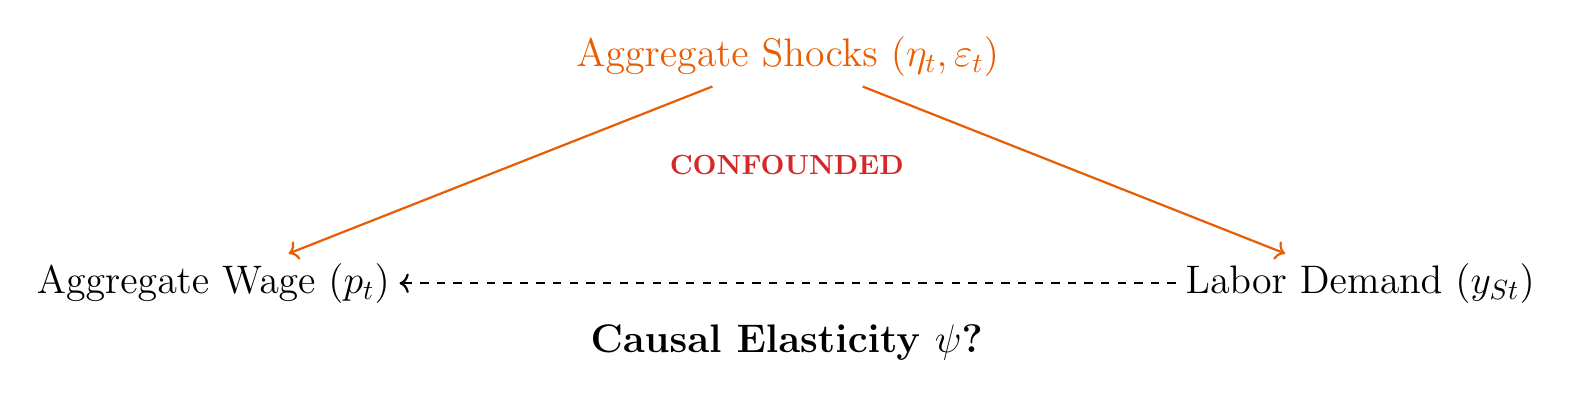
\begin{tikzpicture}[node distance=3cm, font=\Large]
    % Nodes
    \node (agg) [text=WarmOrange] {Aggregate Shocks ($\eta_t, \varepsilon_t$)};
    \node (wage) [below left=of agg] {Aggregate Wage ($p_t$)};
    \node (demand) [below right=of agg] {Labor Demand ($y_{St}$)};
    
    % Paths
    \draw[->, thick, WarmOrange] (agg) -- (wage);
    \draw[->, thick, WarmOrange] (agg) -- (demand);
    \draw[->, thick, dashed] (demand) -- (wage);
    \node[below=0.4cm of $(wage)!0.5!(demand)$] (elasticity) {\textbf{Causal Elasticity $\psi$?}};
    
    % Label for confusion
    \node at ($(wage)!0.5!(demand) + (0, 1.5)$) [text=DeepRed, font=\bfseries] {CONFOUNDED};
\end{tikzpicture}
\end{adjustbox}
\end{center}
\end{frame}

\begin{frame}
\frametitle{Roadmap: From intuition to GMM estimation}
\vspace{0.8cm}
\begin{enumerate}
    \item \textbf{Act II, Sec 1:} The Simple Model — Difference-in-averages.
    \item \textbf{Act II, Sec 2:} The Full Model — Heterogeneous factor loadings.
    \item \textbf{Act II, Sec 3:} Implementation — Python construction and GMM.
    \item \textbf{Act II, Sec 4:} Application — Superstar firms and wage spillovers.
\end{enumerate}
\end{frame}

% --- ACT II, SECTION 1: THE SIMPLE MODEL ---
\transitionslide{Section 1: The Simple Model}{Difference-in-averages as an instrument}

\begin{frame}
\frametitle{Suppose Apple has a breakthrough, but tech is stagnant}
\vspace{1cm}
{\Large
Apple's idiosyncratic success ($u_{it}$) creates a labor demand shock.
}
\vspace{1cm}
{\Large
This shock is \textbf{uncorrelated} with macro-shocks, making it a potential instrument for aggregate prices.
}
\end{frame}

\begin{frame}
\frametitle{Isolating the granular shock via size-weighting}
\vspace{0.5cm}
{\Large
The GIV ($z_t$) is the size-weighted average minus the equal-weighted average.
}
\vspace{1cm}
\begin{equation*}
z_t = \underbrace{\sum S_i y_{it}}_{\text{Size-Weighted}} - \underbrace{\frac{1}{N} \sum y_{it}}_{\text{Equal-Weighted}}
\end{equation*}
\vspace{0.5cm}
{\Large
If $y_{it} = \phi p_t + \eta_t + u_{it}$, then $z_t = u_{St} - u_{Et}$.
}
\end{frame}

\begin{frame}
\frametitle{Subtracting the average "kills" the common factor}
\vspace{0.5cm}
\begin{center}
\begin{adjustbox}{max width=\textwidth}
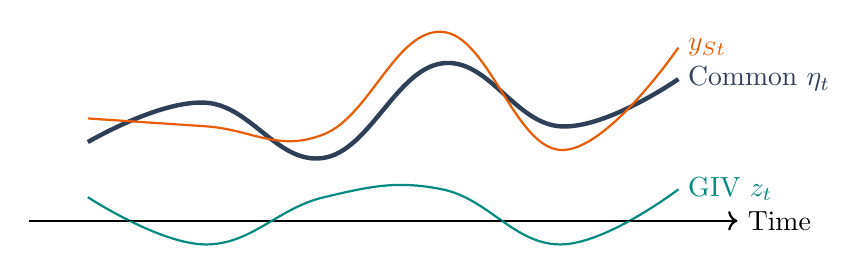
\begin{tikzpicture}[xscale=1.5]
    % Time axis
    \draw[->, thick] (0,0) -- (6,0) node[right] {Time};
    
    % Common factor (eta)
    \draw[DeepNavy, ultra thick] plot[smooth, tension=0.7] coordinates {(0.5,1) (1.5,1.5) (2.5,0.8) (3.5,2) (4.5,1.2) (5.5,1.8)};
    \node[DeepNavy, right] at (5.5,1.8) {Common $\eta_t$};
    
    % y_St (Size-weighted) - similar to eta but with extra jitter
    \draw[WarmOrange, thick] plot[smooth, tension=0.7] coordinates {(0.5,1.3) (1.5,1.2) (2.5,1.1) (3.5,2.4) (4.5,0.9) (5.5,2.2)};
    \node[WarmOrange, right] at (5.5,2.2) {$y_{St}$};
    
    % GIV z_t (Centered around zero)
    \draw[Teal, thick] plot[smooth, tension=0.7] coordinates {(0.5,0.3) (1.5,-0.3) (2.5,0.3) (3.5,0.4) (4.5,-0.3) (5.5,0.4)};
    \node[Teal, right] at (5.5,0.4) {GIV $z_t$};
    
    \draw[dashed] (0,0) -- (6,0);
\end{tikzpicture}
\end{adjustbox}
\end{center}
\end{frame}

% --- ACT II, SECTION 2: THE FULL MODEL ---
\transitionslide{Section 2: The Full Model}{Handling heterogeneous factor loadings}

\begin{frame}
\frametitle{Superstar firms respond differently to macro trends}
\vspace{1cm}
{\Large
The simple GIV ($y_{St} - y_{Et}$) assumes every firm has the same loading $\lambda_i = 1$.
}
\vspace{1cm}
{\Large
If large firms are more sensitive to the Fed, the simple GIV is \textbf{"leaky"}—it correlates with $\eta_t$.
}
\end{frame}

\begin{frame}
\frametitle{The Full Factor Model for granular firms}
\vspace{0.5cm}
We now allow for heterogeneous loadings $\lambda_i$:
\vspace{0.5cm}
\begin{equation}
y_{it} = \phi p_t + \lambda_i \eta_t + u_{it} \tag{full}
\end{equation}
\vspace{0.5cm}
The simple GIV becomes:
\begin{equation*}
z_t = (\lambda_S - \lambda_E) \eta_t + (u_{St} - u_{Et})
\end{equation*}
\vspace{0.5cm}
{\Large
If $\lambda_S \neq \lambda_E$, the instrument is \textbf{invalid} ($\mathbb{E}[z_t \eta_t] \neq 0$).
}
\end{frame}

\begin{frame}
\frametitle{The Solution: Orthogonal Optimal Weights $\Gamma$}
\vspace{0.5cm}
{\Large
We need weights $\Gamma$ such that the factor components \textbf{cancel exactly}.
}
\vspace{1cm}
\begin{equation*}
\sum_{i=1}^N \Gamma_i \lambda_i = 0 \quad \text{(Orthogonality Condition)}
\end{equation*}
\vspace{0.5cm}
{\Large
This ensures $z_t = \sum \Gamma_i u_{it}$ is purely idiosyncratic.
}
\end{frame}

\begin{frame}
\frametitle{Geometry of GIV: Projecting away from the macro trend}
\vspace{0.5cm}
\begin{center}
\begin{adjustbox}{max width=\textwidth}
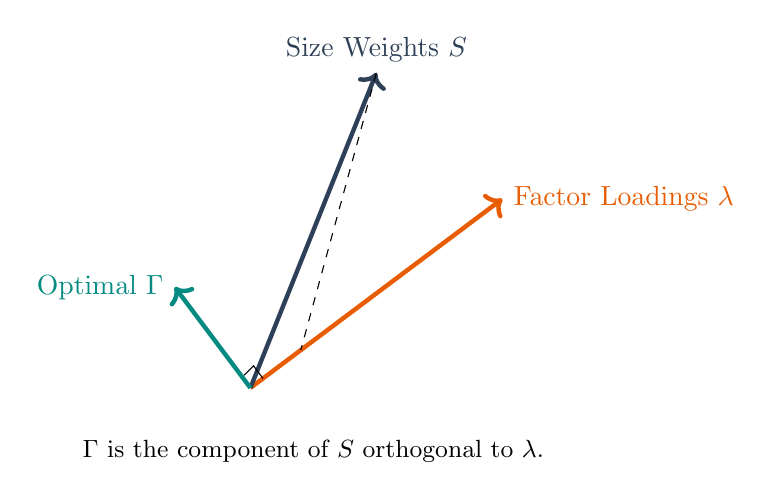
\begin{tikzpicture}[scale=0.8]
    % Vectors
    \draw[->, ultra thick, WarmOrange] (0,0) -- (4,3) node[right] {Factor Loadings $\lambda$};
    \draw[->, ultra thick, DeepNavy] (0,0) -- (2,5) node[above] {Size Weights $S$};
    
    % Projection
    \draw[dashed] (2,5) -- (0.8, 0.6);
    \draw[->, ultra thick, Teal] (0,0) -- (-1.2, 1.6) node[left] {Optimal $\Gamma$};
    
    % Right angle
    \draw (0.2,0.15) -- (0.05, 0.35) -- (-0.1, 0.2);
    
    \node at (1,-1) [font=\small] {$\Gamma$ is the component of $S$ orthogonal to $\lambda$.};
\end{tikzpicture}
\end{adjustbox}
\end{center}
\end{frame}

% --- ACT II, SECTION 3: IMPLEMENTATION ---
\transitionslide{Section 3: Implementation}{Python construction and GMM estimation}

\begin{frame}[fragile]
\frametitle{Constructing the GIV in Python}
\begin{lstlisting}
def construct_giv(df, size_col, outcome_col):
    # 1. Weights
    df['S'] = df[size_col] / df.groupby('year')[size_col].transform('sum')
    df['E'] = 1.0 / df.groupby('year')['id'].transform('count')
    
    # 2. Simple GIV
    y_S = (df[outcome_col] * df['S']).groupby('year').sum()
    y_E = (df[outcome_col] * df['E']).groupby('year').sum()
    z = y_S - y_E
    
    return z
\end{lstlisting}
\end{frame}

\begin{frame}
\frametitle{GMM identifies the model when $\lambda$ is unknown}
\vspace{0.5cm}
{\Large
In practice, we estimate $\phi$ and $\lambda_i$ simultaneously via GMM.
}
\vspace{1cm}
The moment conditions:
\begin{equation*}
\mathbb{E} \left[ (y_{it} - \phi p_t - \lambda_i \eta_t) \cdot z_t \right] = 0
\end{equation*}
\vspace{0.5cm}
{\Large
We use the "Granular Residual" of the largest firms as our source of variation.
}
\end{frame}

\begin{frame}
\frametitle{Strength increases with concentration and micro-volatility}
\vspace{0.2cm}
\begin{center}
    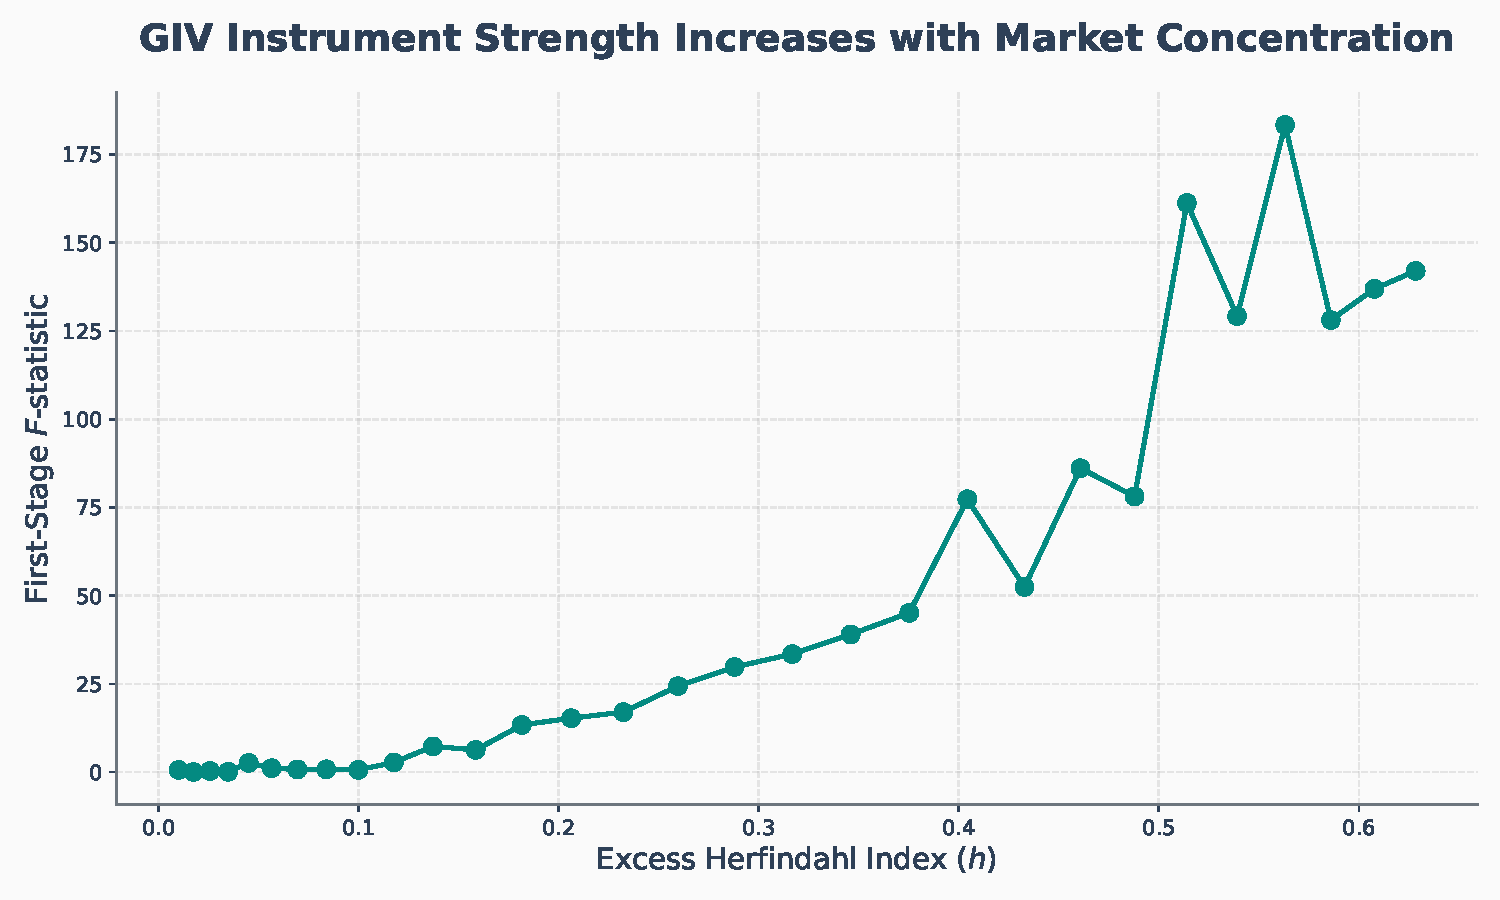
\includegraphics[width=0.75\textwidth]{giv_concentration.pdf}
\end{center}
\end{frame}

% --- ACT II, SECTION 4: LABOR APPLICATION ---
\transitionslide{Section 4: Labor Market Application}{Superstar firms and wage spillovers}

\begin{frame}
\frametitle{Superstar firms drive local wage dynamics}
\vspace{1cm}
{\Large
When Amazon enters a city, its idiosyncratic demand shock ($u_{Amazon, t}$) shifts the aggregate labor demand.
}
\vspace{1cm}
{\Large
GIV identifies the \textbf{General Equilibrium} response of local wages to this granular shift.
}
\end{frame}

\begin{frame}
\frametitle{Devil's Advocate: Are shocks truly idiosyncratic?}
\vspace{0.5cm}
{\Large
A skeptic would say: "Amazon's shock is just a hidden tech-sector trend."
}
\vspace{1cm}
\textbf{The GIV Defense:}
\begin{itemize}
    \item Include industry-year fixed effects (Common Factors).
    \item Use Narrative Checks (e.g., specific policy wins or product failures).
    \item Overidentification tests across size bins.
\end{itemize}
\end{frame}

% --- ACT III: RESOLUTION ---

\begin{frame}
\frametitle{GIV provides a bridge from micro data to macro identification}
\vspace{1cm}
{\Large
We no longer need to search for natural experiments in the aggregate data.
}
\vspace{1cm}
{\Large
The experiments are happening every day at the firm level—we just need to aggregate them correctly.
}
\end{frame}

\begin{frame}[plain]
\vfill
\begin{center}
    {\huge\bfseries\textcolor{DeepNavy}{Large firms' idiosyncratic shocks provide a valid, granular instrument to identify aggregate elasticities.}}
\end{center}
\vfill
\end{frame}

\end{document}
